\documentclass{article}
\usepackage{import}
\documentclass{article}
\usepackage[paper=letterpaper,margin=2cm]{geometry}
\usepackage[utf8]{inputenc}
\usepackage[russian]{babel}
\usepackage[]{graphicx}
\usepackage[usenames]{color}
\usepackage{colortbl}
\usepackage{geometry}
\usepackage{xcolor}
\usepackage{hyperref}
\usepackage{../../lib/latex/listings-rust}
\usepackage{fontspec}
\setmonofont{JetBrains Mono}[Contextuals=Alternate,Ligatures = TeX,]
\usepackage{listings}
\usepackage{keycommand}
\usepackage{caption}

\setmainfont[
  Ligatures=TeX,
  Extension=.otf,
  BoldFont=cmunbx,
  ItalicFont=cmunti,
  BoldItalicFont=cmunbi,
]{cmunrm}
\setsansfont[
  Ligatures=TeX,
  Extension=.otf,
  BoldFont=cmunsx,
  ItalicFont=cmunsi,
]{cmunss}

\geometry{
  a4paper,
  top=25mm,
  right=30mm,
  bottom=25mm,
  left=30mm
}

\hypersetup{
  colorlinks=true,
  linkcolor=blue!50!red,
  urlcolor=blue!70!black
}

\captionsetup[lstlisting]{
  font={tt},
}

% based on Atom One Light
\lstset{
  language=Java,
  frame=single,
  basicstyle=\ttfamily\color[HTML]{383a42},
  columns=fullflexible,
  breaklines=true,
  numbers=left,
  frame=tab,
  postbreak=\mbox{\textcolor{red}{$\hookrightarrow$}\space},
  extendedchars=false,
  showspaces=false,
  showstringspaces=false,
  identifierstyle=\ttfamily\color[HTML]{4078f2},
  commentstyle=\color[HTML]{a0a1a7},
  stringstyle=\color[HTML]{50a14f},
  keywordstyle=\color[HTML]{a626a4},
  numberstyle=\ttfamily\color[HTML]{2c91af},
  rulecolor=\color[HTML]{383a42}
}

\lstdefinelanguage{XML}
{
  morestring=[b]",
  morestring=[s]{>}{<},
  morecomment=[s]{<?}{?>},
}

\newcommand{\code}[1]{
  \lstset{title=#1}
  \lstinputlisting{#1}
}
\newkeycommand{\itmo}[variant=aboba, labn=aboba, discipline=aboba, group=aboba, student=aboba,teacher=aboba, year=2022]{
  \begin{titlepage}
    \begin{center}
      \section*{
        Федеральное государственное автономное образовательное учреждение\\ высшего образования\\
        «Национальный исследовательский университет ИТМО»\\
        Факультет Программной Инженерии и Компьютерной Техники \\
       }
      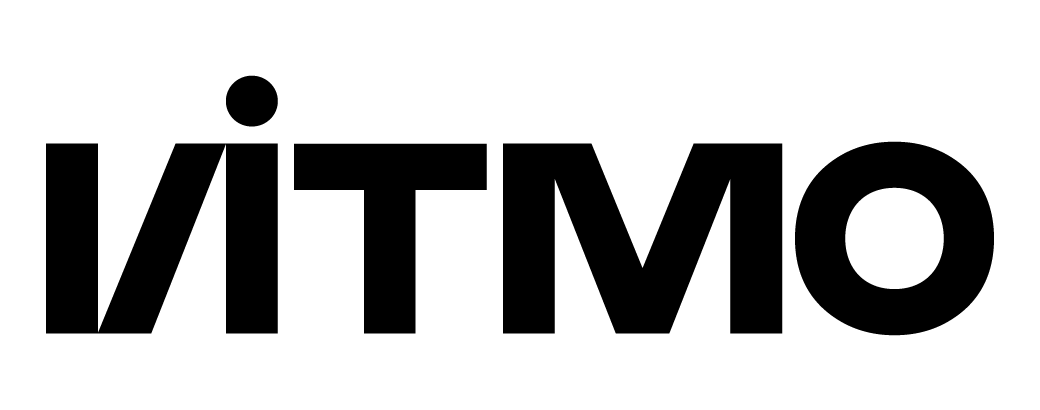
\includegraphics[scale=0.2]{../../lib/img/itmo.png}
    \end{center}

    \vspace{4cm}

    \begin{center}
      \large \textbf{Вариант \textnumero \commandkey{variant}}\\
      \textbf{Лабораторная работа \textnumero \commandkey{labn}}\\
      по дисциплине\\
      \textbf{\commandkey{discipline}}
    \end{center}

    \vspace*{\fill}

    \begin{flushright}
      Выполнил Студент группы \commandkey{group}\\
      \textbf{\commandkey{student}}\\
      Преподаватель: \\
      \textbf{\commandkey{teacher}}\\
    \end{flushright}

    \vspace{1cm}

    \begin{center}
      г. Санкт-Петербург\\
      \commandkey{year}г.
    \end{center}

    \thispagestyle{empty}
  \end{titlepage}
}



\begin{document}

\itmo[
  variant=1513,
  labn=2,
  discipline=Информационные системы и базы данных,
  group=P3115,
  student=Владимир Мацюк,
  teacher=Горбунов Михаил Витальевич,
  year=2023,
  logo=../../lib/img/itmo.png
]

\section{Текст задания}
\begin{enumerate}
  \item Сделать запрос для получения атрибутов из указанных таблиц, применив фильтры по указанным условиям:
        Н\_ТИПЫ\_ВЕДОМОСТЕЙ, Н\_ВЕДОМОСТИ.
        Вывести атрибуты: Н\_ТИПЫ\_ВЕДОМОСТЕЙ.ИД, Н\_ВЕДОМОСТИ.ЧЛВК\_ИД.
        Фильтры (AND):
        a) Н\_ТИПЫ\_ВЕДОМОСТЕЙ.ИД < 3.
        b) Н\_ВЕДОМОСТИ.ЧЛВК\_ИД > 163249.
        Вид соединения: LEFT JOIN.
  \item Сделать запрос для получения атрибутов из указанных таблиц, применив фильтры по указанным условиям:
        Таблицы: Н\_ЛЮДИ, Н\_ВЕДОМОСТИ, Н\_СЕССИЯ.
        Вывести атрибуты: Н\_ЛЮДИ.ОТЧЕСТВО, Н\_ВЕДОМОСТИ.ЧЛВК\_ИД, Н\_СЕССИЯ.ДАТА.
        Фильтры (AND):
        a) Н\_ЛЮДИ.ИМЯ > Роман.
        b) Н\_ВЕДОМОСТИ.ДАТА = 2010-06-18.
        c) Н\_СЕССИЯ.УЧГОД < 2003/2004.
        Вид соединения: INNER JOIN.
  \item Вывести число студентов вечерней формы обучения, которые не имеет отчества.
        Ответ должен содержать только одно число.
  \item В таблице Н\_ГРУППЫ\_ПЛАНОВ найти номера планов, по которым обучается (обучалось) менее 2 групп на заочной форме обучения.
        Для реализации использовать соединение таблиц.
  \item   Выведите таблицу со средними оценками студентов группы 4100 (Номер, ФИО, Ср\_оценка), у которых средняя оценка меньше средней оценк(е|и) в группе 1101.
        Получить список студентов, зачисленных до первого сентября 2012 года на первый курс заочной формы обучения (специальность: Программная инженерия). В результат включить:
        номер группы;
        номер, фамилию, имя и отчество студента;
        номер и состояние пункта приказа;
        Для реализации использовать подзапрос с IN.
  \item Вывести список студентов, имеющих одинаковые фамилии, но не совпадающие ид.
\end{enumerate}
\lstset{language=SQL}
\begin{enumerate}
  \item \begin{lstlisting}
  select "Н_ТИПЫ_ВЕДОМОСТЕЙ"."ИД" as "Н_ТИПЫ_ВЕДОМОСТЕЙ.ИД",
  "Н_ВЕДОМОСТИ"."ЧЛВК_ИД"  as "Н_ВЕДОМОСТИ.ЧЛВК_ИД"
from "Н_ВЕДОМОСТИ"
    left join "Н_ТИПЫ_ВЕДОМОСТЕЙ" on "Н_ТИПЫ_ВЕДОМОСТЕЙ"."ИД" = "Н_ВЕДОМОСТИ"."ТВ_ИД"
where "Н_ТИПЫ_ВЕДОМОСТЕЙ"."ИД" < 3
and "Н_ВЕДОМОСТИ"."ЧЛВК_ИД" > 163249;
\end{lstlisting}
        
        
  \item \begin{lstlisting}
    select "Н_ЛЮДИ"."ОТЧЕСТВО", "Н_ВЕДОМОСТИ"."ЧЛВК_ИД", "Н_СЕССИЯ"."ДАТА"
    from "Н_ЛЮДИ"
             inner join "Н_ВЕДОМОСТИ" on "Н_ЛЮДИ"."ИД" = "Н_ВЕДОМОСТИ"."ЧЛВК_ИД"
             inner join "Н_СЕССИЯ" on "Н_ВЕДОМОСТИ"."ЧЛВК_ИД" = "Н_СЕССИЯ"."ЧЛВК_ИД"
    where "Н_ЛЮДИ"."ИМЯ" > 'Роман'
      and "Н_ВЕДОМОСТИ"."ДАТА" = '2010-06-18'
      and "Н_СЕССИЯ"."УЧГОД" < '2003 / 2004'
    
\end{lstlisting}
        
  \item \begin{lstlisting}
  select count(*)
  from "Н_УЧЕНИКИ"
           inner join "Н_ЛЮДИ" on "Н_УЧЕНИКИ"."ЧЛВК_ИД" = "Н_ЛЮДИ"."ИД"
           inner join "Н_ПЛАНЫ" on "Н_УЧЕНИКИ"."ПЛАН_ИД" = "Н_ПЛАНЫ"."ПЛАН_ИД"
           inner join "Н_ФОРМЫ_ОБУЧЕНИЯ" on "Н_ПЛАНЫ"."ФО_ИД" = "Н_ФОРМЫ_ОБУЧЕНИЯ"."ИД"
      and "ИМЯ_В_ИМИН_ПАДЕЖЕ" = 'очная'
  where "ОТЧЕСТВО" is null
\end{lstlisting}
        
        
  \item \begin{lstlisting}
  select
  "Н_ГРУППЫ_ПЛАНОВ"."ПЛАН_ИД"
from "Н_ГРУППЫ_ПЛАНОВ"
       join (select count(*) as cnt, "ГРУППА"
             from "Н_ГРУППЫ_ПЛАНОВ"
             group by "ГРУППА") as ggg on "Н_ГРУППЫ_ПЛАНОВ"."ГРУППА" = ggg."ГРУППА"

       join "Н_ПЛАНЫ" on "Н_ГРУППЫ_ПЛАНОВ"."ПЛАН_ИД" = "Н_ПЛАНЫ"."ПЛАН_ИД"
       join "Н_ФОРМЫ_ОБУЧЕНИЯ"
            on "Н_ФОРМЫ_ОБУЧЕНИЯ"."ИД" = "Н_ПЛАНЫ"."ФО_ИД" and "НАИМЕНОВАНИЕ" = 'Заочная'
where cnt < 2
\end{lstlisting}
        
        
        
  \item \begin{lstlisting}
    select "Н_ЛЮДИ"."ИД"               as "Номер",
    CONCAT(' ', "Н_ЛЮДИ"."ФАМИЛИЯ", ' ', "Н_ЛЮДИ"."ИМЯ", ' ',
           "Н_ЛЮДИ"."ОТЧЕСТВО") as "ФИО",
    "Ср_оценка"
from (select avg(CASE
                  WHEN "Н_ВЕДОМОСТИ"."ОЦЕНКА" ~ E'^\\d+$' THEN
                      CAST("Н_ВЕДОМОСТИ"."ОЦЕНКА" AS INTEGER)
 END) as "Ср_оценка",
          "Н_УЧЕНИКИ"."ИД"
   from "Н_ВЕДОМОСТИ"
            inner join "Н_УЧЕНИКИ" on "Н_ВЕДОМОСТИ"."ЧЛВК_ИД" = "Н_УЧЕНИКИ"."ЧЛВК_ИД" and "ГРУППА" = '4100'
   group by "Н_УЧЕНИКИ"."ИД") as ids
      join "Н_УЧЕНИКИ" on ids."ИД" = "Н_УЧЕНИКИ"."ИД"
      join "Н_ЛЮДИ" on "Н_ЛЮДИ"."ИД" = "ЧЛВК_ИД"
where "Ср_оценка" > (select avg(CASE
                                 WHEN "Н_ВЕДОМОСТИ"."ОЦЕНКА" ~ E'^\\d+$' THEN
                                     CAST("Н_ВЕДОМОСТИ"."ОЦЕНКА" AS INTEGER)
 END)
                  from "Н_ВЕДОМОСТИ"
                           inner join "Н_УЧЕНИКИ"
                                      on "Н_ВЕДОМОСТИ"."ЧЛВК_ИД" = "Н_УЧЕНИКИ"."ЧЛВК_ИД" and "ГРУППА" = '1101');
\end{lstlisting}
        
        
  \item \begin{lstlisting}
    SELECT "Н_УЧЕНИКИ"."ГРУППА"                                         AS "Номер группы",
    CONCAT("Н_ЛЮДИ"."ИД", ' ', "Н_ЛЮДИ"."ФАМИЛИЯ", ' ', "Н_ЛЮДИ"."ИМЯ", ' ',
           "Н_ЛЮДИ"."ОТЧЕСТВО")                                  AS "Номер, фамилия, имя и отчество студента",
    CONCAT("Н_УЧЕНИКИ"."П_ПРКОК_ИД", ' ', "Н_УЧЕНИКИ"."ПРИЗНАК") AS "Номер и состояние пункта приказа"
FROM "Н_УЧЕНИКИ"
      JOIN "Н_ЛЮДИ" ON "Н_ЛЮДИ"."ИД" = "Н_УЧЕНИКИ"."ЧЛВК_ИД"
WHERE "Н_УЧЕНИКИ"."НАЧАЛО"::date < '2012-09-01'
AND "Н_УЧЕНИКИ"."ПЛАН_ИД" IN (SELECT "Н_ПЛАНЫ"."ИД"
                             FROM "Н_ПЛАНЫ"
                                      JOIN "Н_ФОРМЫ_ОБУЧЕНИЯ" ON "Н_ФОРМЫ_ОБУЧЕНИЯ"."ИД" = "Н_ПЛАНЫ"."ФО_ИД" AND
                                                                 "Н_ФОРМЫ_ОБУЧЕНИЯ"."НАИМЕНОВАНИЕ" =
                                                                 'Очно-заочная(вечерняя)'
                                      JOIN "Н_НАПРАВЛЕНИЯ_СПЕЦИАЛ"
                                           ON "Н_ПЛАНЫ"."НАПС_ИД" = "Н_НАПРАВЛЕНИЯ_СПЕЦИАЛ"."ИД"
                                      JOIN "Н_НАПР_СПЕЦ" ON "Н_НАПРАВЛЕНИЯ_СПЕЦИАЛ"."НС_ИД" = "Н_НАПР_СПЕЦ"."ИД"
                                 AND "Н_НАПР_СПЕЦ"."НАИМЕНОВАНИЕ" =
                                     'Вычислительные машины, комплексы, системы и сети');
\end{lstlisting}
        
        
        
  \item \begin{lstlisting}
    select "Н_ЛЮДИ"."ИД"               as "Номер",
    CONCAT(' ', "Н_ЛЮДИ"."ФАМИЛИЯ", ' ', "Н_ЛЮДИ"."ИМЯ", ' ',
           "Н_ЛЮДИ"."ОТЧЕСТВО") as "ФИО"
from "Н_УЧЕНИКИ"
      join "Н_ЛЮДИ" on "Н_УЧЕНИКИ"."ЧЛВК_ИД" = "Н_ЛЮДИ"."ИД"
where "ФАМИЛИЯ" in (select "ФАМИЛИЯ"
                 from "Н_ЛЮДИ"
                 group by "ФАМИЛИЯ"
                 having count("ФАМИЛИЯ") > 1
                 order by "ФАМИЛИЯ")
group by "Н_ЛЮДИ"."ИД", "Н_ЛЮДИ"."ФАМИЛИЯ", "Н_ЛЮДИ"."ИМЯ",
      "Н_ЛЮДИ"."ОТЧЕСТВО"
order by "ФИО"
\end{lstlisting}
        
        
\end{enumerate}

\section{Вывод}
Во время выполнения работы я узеал больше про SQL.
\end{document}
